\chapter{Paparazzi Center}

% TODO: ¿Sección de instalación?

\noindent Una vez realizada la instalación, podremos ejecutar el binario precompilado \textit{paparazzi} que se encuentra en la carpeta raíz de Paparazzi. Entonces se inicializará todo el ecosistema y se ejecutará Paparazzi Center, el panel de control principal de PaparazziUAV [Figura \ref{fig:cap1_interfaz}]. En él nos encontraremos inicialmente con un proyecto (A/C) ejemplo. Dentro de cada proyecto podremos introducir varios \textbf{archivos de configuración .xml} (en el capítulo sobre el directorio \textit{conf} explicaremos más detalladamente para qué sirve cada uno):

\begin{enumerate}
    \item \textbf{Airframe}: va a contener toda la información sobre el hardware y firmware de nuestro vehículo. \url{https://wiki.paparazziuav.org/wiki/Airframe_Configuration}.
    
    \item \textbf{Flight Plan}: definirá la geolocalización, los bloques y los waypoints que aparecerán en el modo navegación.
    
    \item \textbf{Radio}: ajustará las ganancias y la funcionalidad de los canales del radio control. Paparazzi ya trae la configuración de varios modelos, si nuestro controlador no se encuentra entre ellos deberemos de generar su .xml teniendo en cuenta sus especificaciones.
    
    \item \textbf{Telemetry}: definirá los distintos modos de telemetría del vehículo y los mensajes que se enviarán en cada uno de ellos. 
    
\end{enumerate}

\begin{figure}[h!]
    \centering
    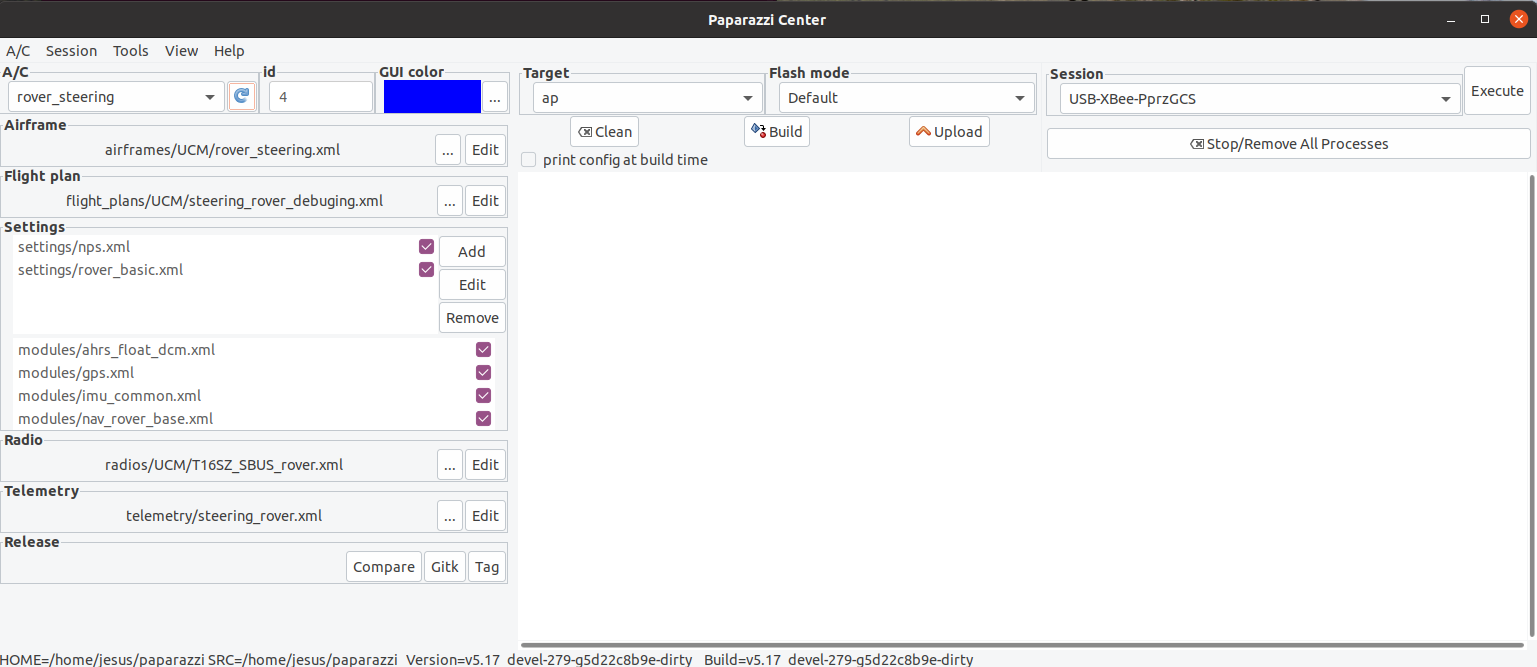
\includegraphics[width=0.8\textwidth]{./figuras/cap1_interfaz.png}
    \caption{Interfaz de Paparazzi Center, el panel de control principal de PaparazziUAV.} \label{fig:cap1_interfaz}
\end{figure}

\newpage

Para compilar ... \\

Herramientas y sesiones ... \\

